%!TEX encoding = UTF-8 Unicode

% this figure should come before the proposed approach section.
% It might happen automatically if we shorten the introduction.
% Otherwise move back in the files.
\begin{figure*}
  \centering
  \subfloat[]{
    \resizebox{\linewidth}{!}{
      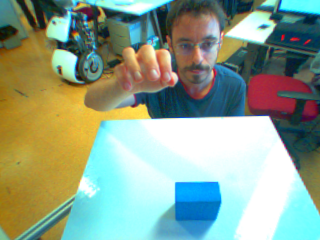
\includegraphics{grasp-00000169}
      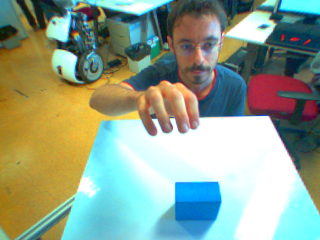
\includegraphics{grasp-00000170}
      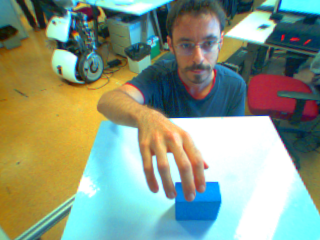
\includegraphics{grasp-00000171}
      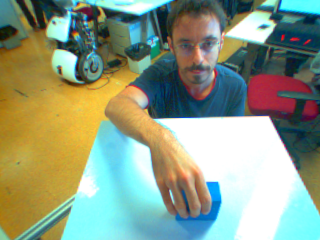
\includegraphics{grasp-00000173}
      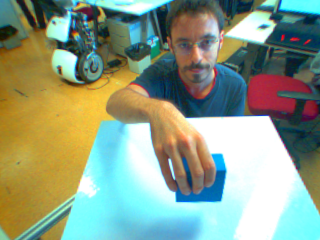
\includegraphics{grasp-00000177}
      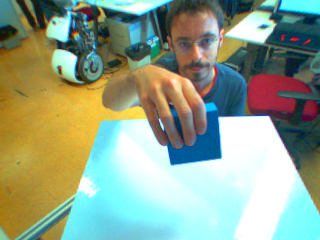
\includegraphics{grasp-00000180}
    } % end resizebox
    \label{fig:action_examples:grasp}
  } % end subfloat

  \subfloat[]{
    \resizebox{\linewidth}{!}{
      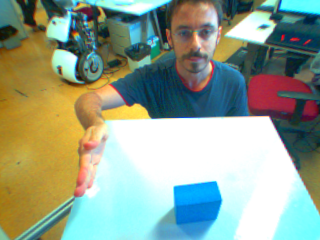
\includegraphics{tap-00000109}
      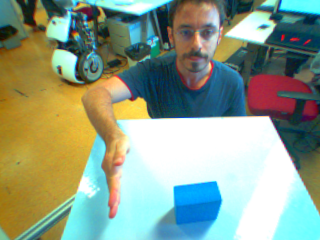
\includegraphics{tap-00000110}
      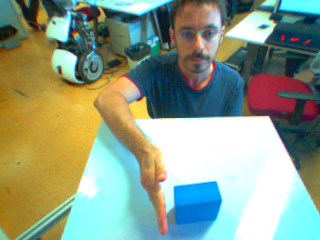
\includegraphics{tap-00000112}
      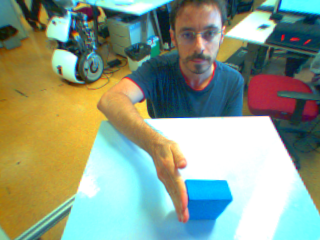
\includegraphics{tap-00000114}
      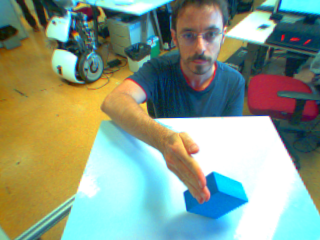
\includegraphics{tap-00000116}
      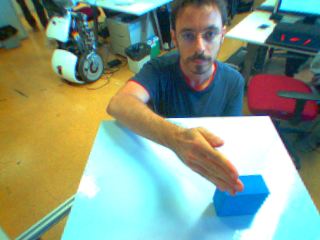
\includegraphics{tap-00000117}
    } % end resizebox
    \label{fig:action_examples:tap}
  } % end subfloat

  \subfloat[]{
    \resizebox{\linewidth}{!}{
      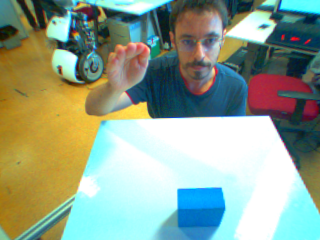
\includegraphics{touch-00000196}
      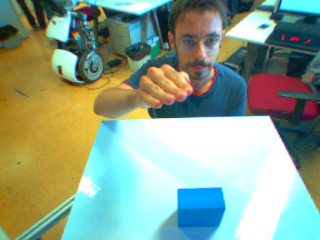
\includegraphics{touch-00000197}
      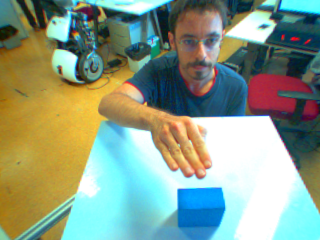
\includegraphics{touch-00000198}
      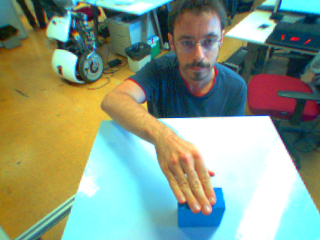
\includegraphics{touch-00000200}
      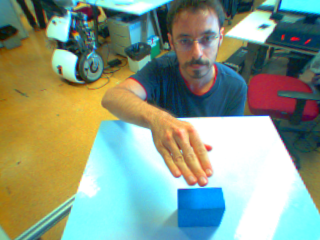
\includegraphics{touch-00000202}
      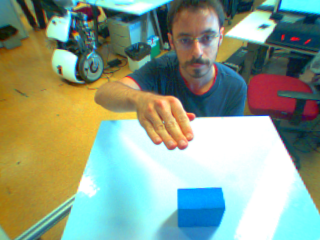
\includegraphics{touch-00000203}
    } % end resizebox
    \label{fig:action_examples:touch}
  } % end subfloat
  \caption{Examples of human actions from the point of view of the robot.
  (a)~Grasp action: moving the hand towards an object vertically, then grasping and lifting it.
  (b)~Tap action: moving the hand towards an object laterally then touching it, causing a motion effect.
  (c)~Touch action: moving the hand towards an object vertically, touching it~(without grasping), then retracting the hand.}
  \label{fig:action_examples}
\end{figure*}

\section{Introduction}
\label{sec:intro}

\IEEEPARstart{C}{ooperation}, or the ability of working successfully in groups, is a tenet of human society~\cite{turner:1975}.
This skill is acquired by human children incrementally, around the second year of life, as they develop the ability to coordinate themselves with peers or adult caregivers in shared problem-solving activities and social games~\cite{brownell:2006:childdev}.
This is achieved not only by mere behavioral coordination, but also by employing communicative strategies~\cite{melis:2010:rstb} and by continuously observing partners' actions~\cite{ramnani:2004:natureneuro}.
Loosely inspired by these observations, this paper presents and evaluates a cognitive system for robots which permits reasoning over subsequent phases:
first about self-learned knowledge~(about affordances and language-based descriptions of objects),
and then about others' actions.

Even though social robots\footnote{A social robot is ``[a robot that is] able to communicate and interact with us, understand and even relate to us, in a personal way. [It] should be able to understand us and itself in social terms''~\cite{breazeal:2002:dsr}.} are becoming common in domestic and public environments, \hr{} teams still lag behind \hh{} teams in terms of effectiveness.
For robots, interpreting the actions of others and learning to describe them verbally~(for effective cooperation) is challenging.
The reason is that we cannot possibly model all the imaginable physical, verbal and non-verbal~(e.g., gestures) cues that can take place during \hri, due to the richness of language and the high variability of the real world outside of structured research laboratories and factories.
Hence, it is necessary to have robots that \emph{learn} world elements and properties of language~\cite{iwahashi:2007:hri}, and the ability to link these verbal elements with other skills, such as other perceptual modalities~(e.g., vision of objects and other agents) and manipulation abilities~(e.g., grasping objects and placing them in order to achieve a goal)~\cite{steels:2003:trendscogsci}.

This paper builds upon the intuition that a robot can generalize its previously-acquired knowledge of the world~(e.g., motor actions, objects properties, physical effects, verbal descriptions) to those situations where it observes a human agent performing familiar actions in a shared \hr{} scenario.
We follow the developmental robotics perspective~\cite{lungarella:2003:devrobsurvey,cangelosi:2015:devrobbook},
which takes inspiration from the progressive learning phenomena observed in children's mental development~(e.g., the understanding of language, the acquisition of manipulation skills, the comprehension of others' actions), and investigates how to model the evolution and acquisition of these increasingly complex cognitive processes in artificial autonomous systems.

In particular, we are inspired by the possible existence of a shared representation for self-related and others-related knowledge in the human brain~\cite{gallagher:1996:earliest,rizzolatti:2001:nrn,decety:2003:sharedrep}, and we look at the developmental stages in which human children have consolidated an idea of \selfother{} distinction~\cite{symons:2004:mental} and start to reason about the external world also in allocentric terms~\cite{ribordy:2013:development}, in addition to the ego-centric ones, and could therefore possibly begin to use knowledge about the \emph{self} to infer about \emph{others}.

Extending on our recent work~\cite{saponaro:2017:glu}, in this paper we combine robot ego-centric learning about language and object affordances~\cite{salvi:2012:smcb} with the observation of external agents through gesture recognition~\cite{saponaro:2013:crhri}.
Our novel contributions are as follows.
\begin{enumerate}
\item A probabilistic method to fuse self-learned knowledge of language and object affordances, with socially aware information of others' physical actions~(in the form of uncertain soft evidence).

\item Experimental findings showing the reasoning power of our combined system, which is able to make inferences and predictions over affordances and words.

\item The possibility of generating verbal descriptions from the estimated word probabilities and a pre-defined grammar, with emergence of non-trivial language properties such as congruent/incongruent conjunctions, synonyms between two consecutive sentences speaking about the same concepts.
\end{enumerate}
Furthermore, we make our human action data and probabilistic reasoning code publicly available\footnote{\url{https://github.com/giampierosalvi/AffordancesAndSpeech}: the code from \cite{salvi:2012:smcb} has been extended to support the experiments in this paper.}\footnote{\url{https://github.com/gsaponaro/tcds-gestures}: code from this paper.} in the interest of reproducibility.

This paper is structured as follows.
In Section~\ref{sec:related_work}, we briefly overview the literature on the interpretation and verbal description of others in different disciplines.
In Section~\ref{sec:method}, we present our proposed method and its components.
In Section\ref{sec:experimental_settings}, we provide details and assumptions of the approach.
Section\ref{sec:results} illustrates our results, and
in Section\ref{sec:conclusions}, we draw our concluding remarks.
